%!TEX root = ../my_thesis.tex
\section{Time-dependent selection efficiency}
\label{sec:time:acc}

Because of some of the selection criteria described in Sec.~\ref{sec:sample_and_selection}, the $\Bz$ decay time distribution is biased, \ie~different from the shape it would have with a constant selection efficiency. This efficiency, called here and after ``acceptance'', is a function of the reconstructed proper time. In particular, it goes very rapidly to zero at low decay times due to the impact parameter requirements which exclude short-lived $\Bz$ candidates; then, it reaches a ``plateau'' at intermediate decay times; finally, it drops at high decay times due to the acceptance of the VELO reconstruction. 

The acceptance function $a(t)$ is parameterised using splines defined analytically as described in Ref.~\cite{spline}. These splines are cubic polynomials defined in sub-ranges of the decay time. The boundaries of each sub-range, called ``knots'', are located at 0.4, 0.5, 1.0, 1.5, 2.0, 2.3, 2.6, 3.0, 4.0, 10.0, and 12.0 ps. The location of the 11 knots and the higher density of knots at low decay times, where the acceptance is a strongly-varying function of $t$, ensure that the resulting acceptance is sufficiently smooth. For each knot $t_{i}$, a coefficient $v_{i}$ is defined, which is the actual value of the acceptance function $a(t_{i})$. In order to fix the overall scale of the acceptance function, the $v_{10}$ coefficient is set to 1.0. Moreover, since statistical fluctuations at high decay times may strongly affect $v_{11}$, the latter is constrained to be the linear extrapolation from the previous two coefficients:
\begin{equation}
	v_{11} = v_{10} + \frac{v_{10} - v_{9}}{t_{10}-t_{9}} \times (t_{11}-t_{10})\,.
\end{equation}     

The knot positions and the number of knots are optimized in order to fit the $\Bz\to\Dmp\pipm$ Monte Carlo decay time distribution with sufficient fit quality. The PDF adopted in this fit is proportional to: 
\begin{equation}
	a(t) \int dt' \mathcal R(t-t') e^{-t'/\tau_d},
\end{equation}
where $\mathcal R(t-t')$ is the average resolution model discussed in Sec.~\ref{sec:time:resol} and $\tau_d$ is the $\Bz$ lifetime value used in the Monte Carlo generation. All acceptance coefficients are floating in the fit, while resolution and lifetime are fixed.

The fit projection is shown if Fig.~\ref{fig:AcceptanceFitAll} together with the correlation matrix obtained from the fit, whereas the fitted coefficients are listed in Table~\ref{tab:AcceptanceFitAll}.


\begin{figure}[t]
        \centering
        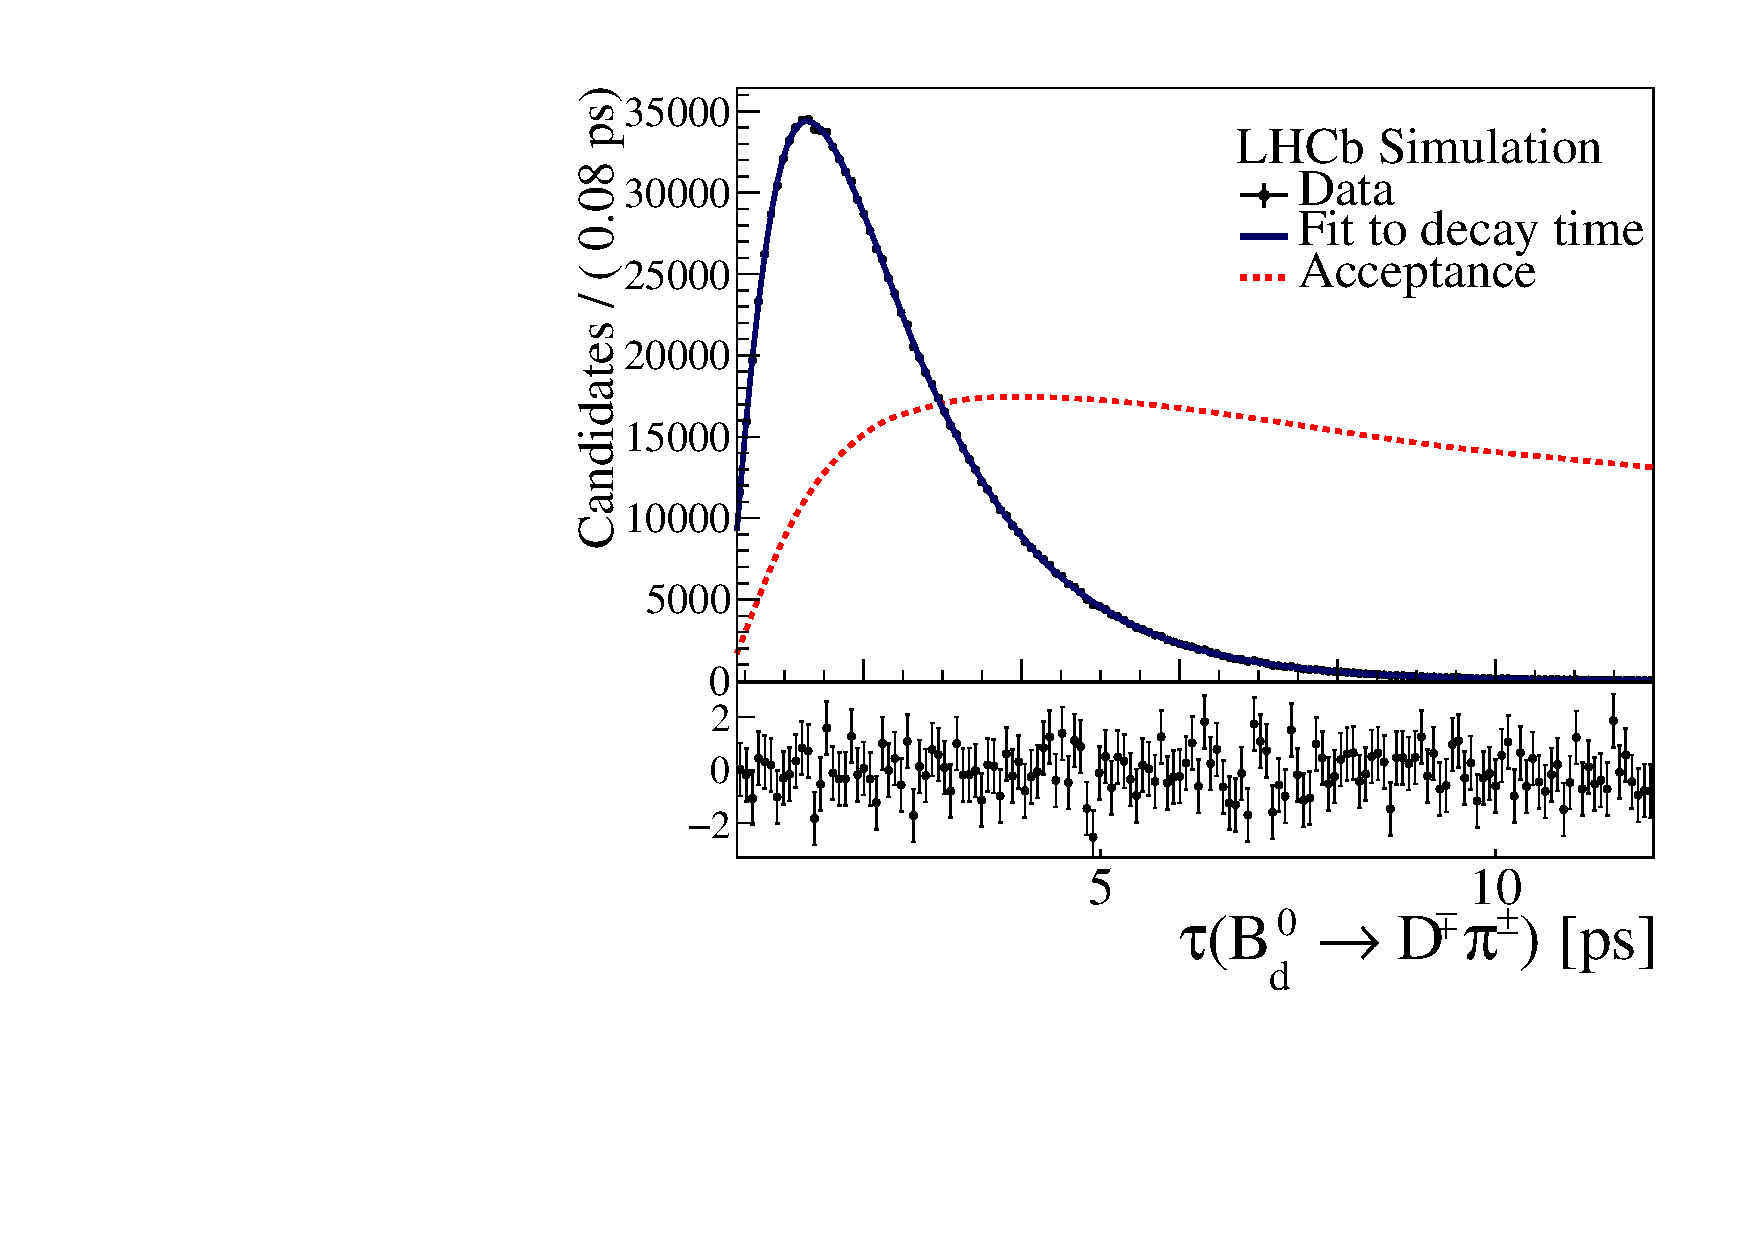
\includegraphics[width=0.44\linewidth]{05DecaytimeFit/figs/MCAcceptance/MCAcceptance.pdf}
        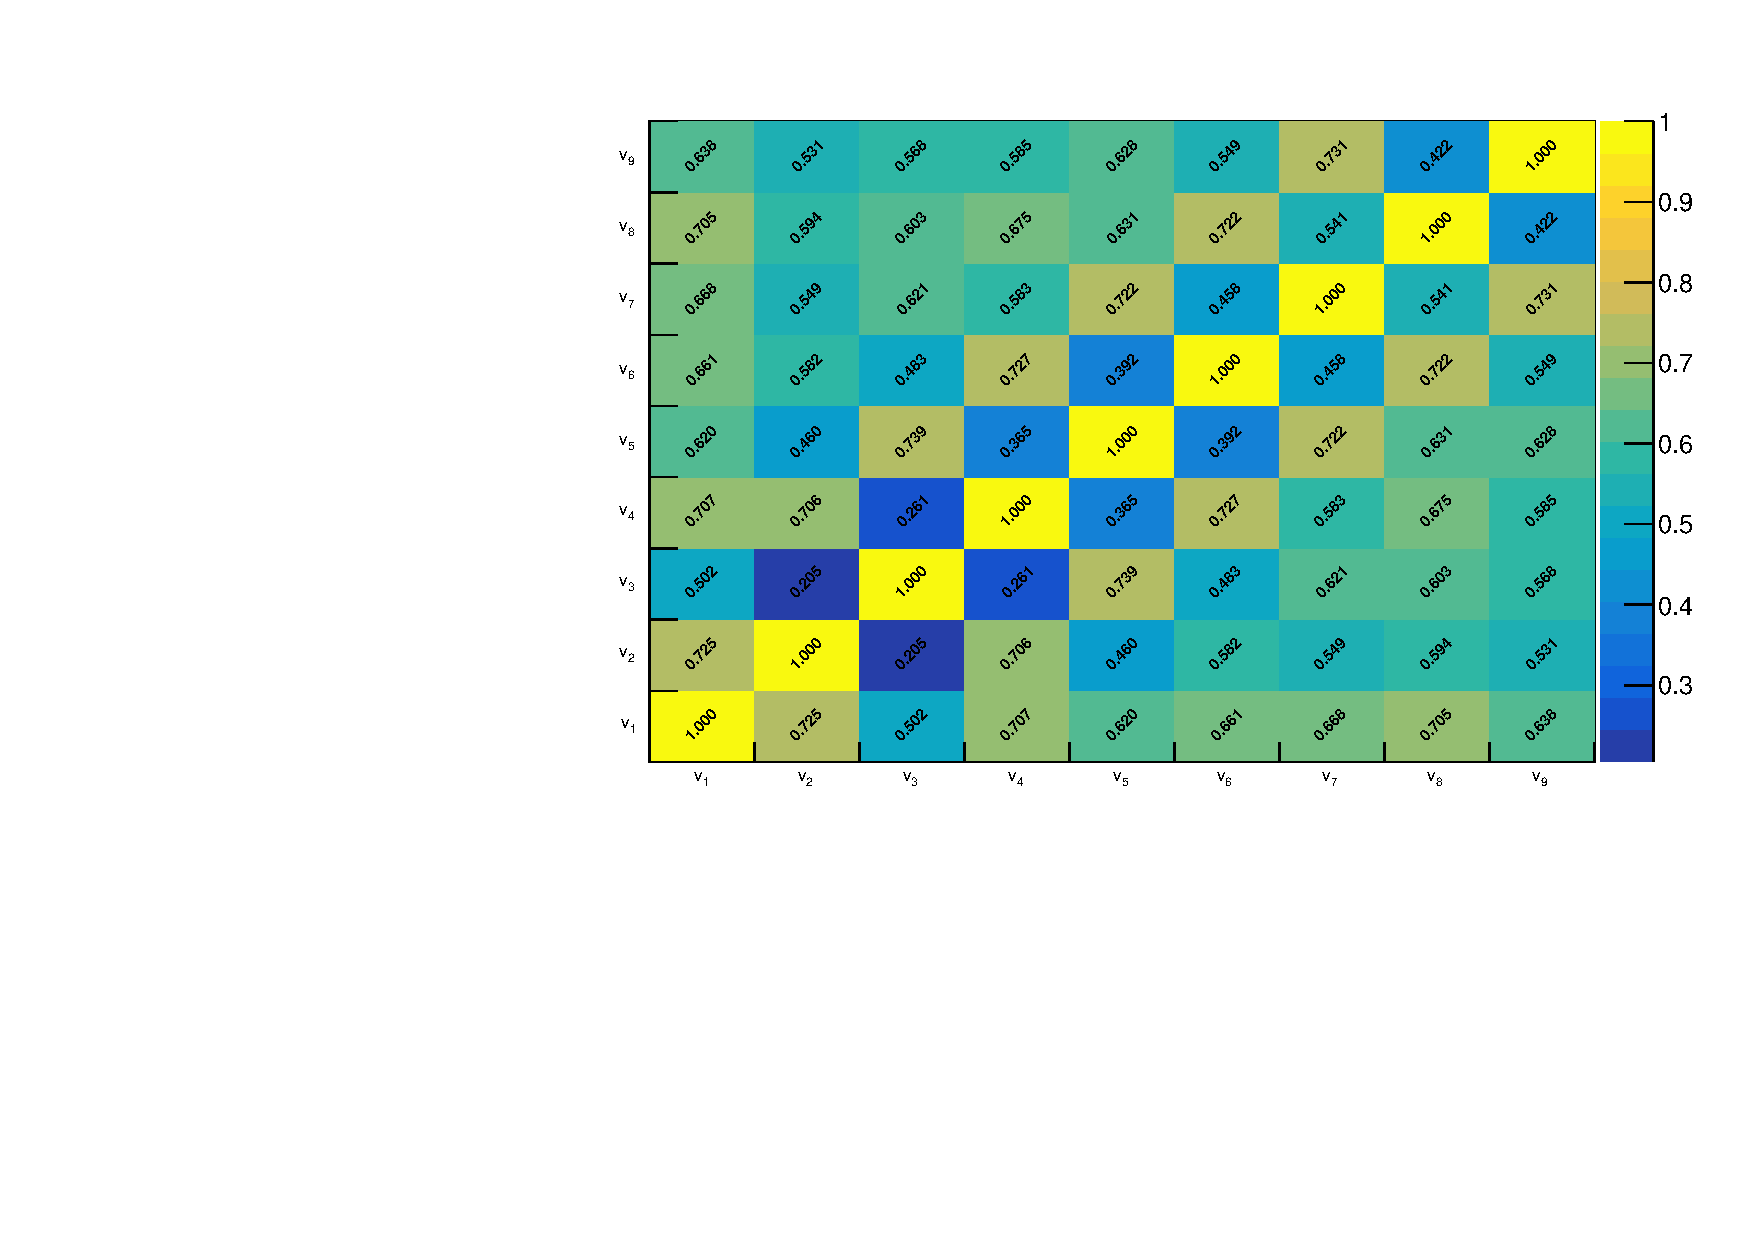
\includegraphics[width=0.52\linewidth]{05DecaytimeFit/figs/MCAcceptance/acceptance_CorrelationMatrix.pdf}
        \vspace{-2mm}
        \caption{Left: distribution of the reconstructed decay time of simulated and selected $\Bz\to\Dmp\pipm$ decays (data points), with fit model superimposed (blue curve), and fitted acceptance function (red dotted curve). Right: correlation matrix of the nine fitted acceptance parameters.}
        \label{fig:AcceptanceFitAll}
\end{figure}

\begin{table}[tb]
\begin{center}
\caption{Acceptance parameters fitted on the signal Monte Carlo sample.}
\begin{tabular}{cc}
\toprule
Parameter name & Fitted value \\
\midrule
$v_{1}$ & $0.1961\pm0.0016$ \\
$v_{2}$ & $0.3348\pm0.0032$ \\
$v_{3}$ & $0.6159\pm0.0057$  \\
$v_{4}$ & $0.8667\pm0.0073$  \\
$v_{5}$ & $0.9982\pm0.0086$  \\
$v_{6}$ & $1.0747\pm0.0091$  \\
$v_{7}$ & $1.1051\pm0.0094$ \\
$v_{8}$ & $1.1590\pm0.0086$ \\
$v_{9}$ & $1.188\pm0.014$ \\
\bottomrule
\end{tabular}
\label{tab:AcceptanceFitAll}
\end{center}
\end{table}
